\newpage
\section{Data-flow and DMA}

Before reading this section keep in mind that this section is a mix of both hardware and software.\\
There are a lot of data what goes through the PSoC, too get a better overview of have the data are measured too the data ends up on the PC a Data-flow diagram has been made. there are both digital and analog filters, and even some down-samplings.

\subsection{Flow diagram}

\begin{figure}[H]
	\centering
	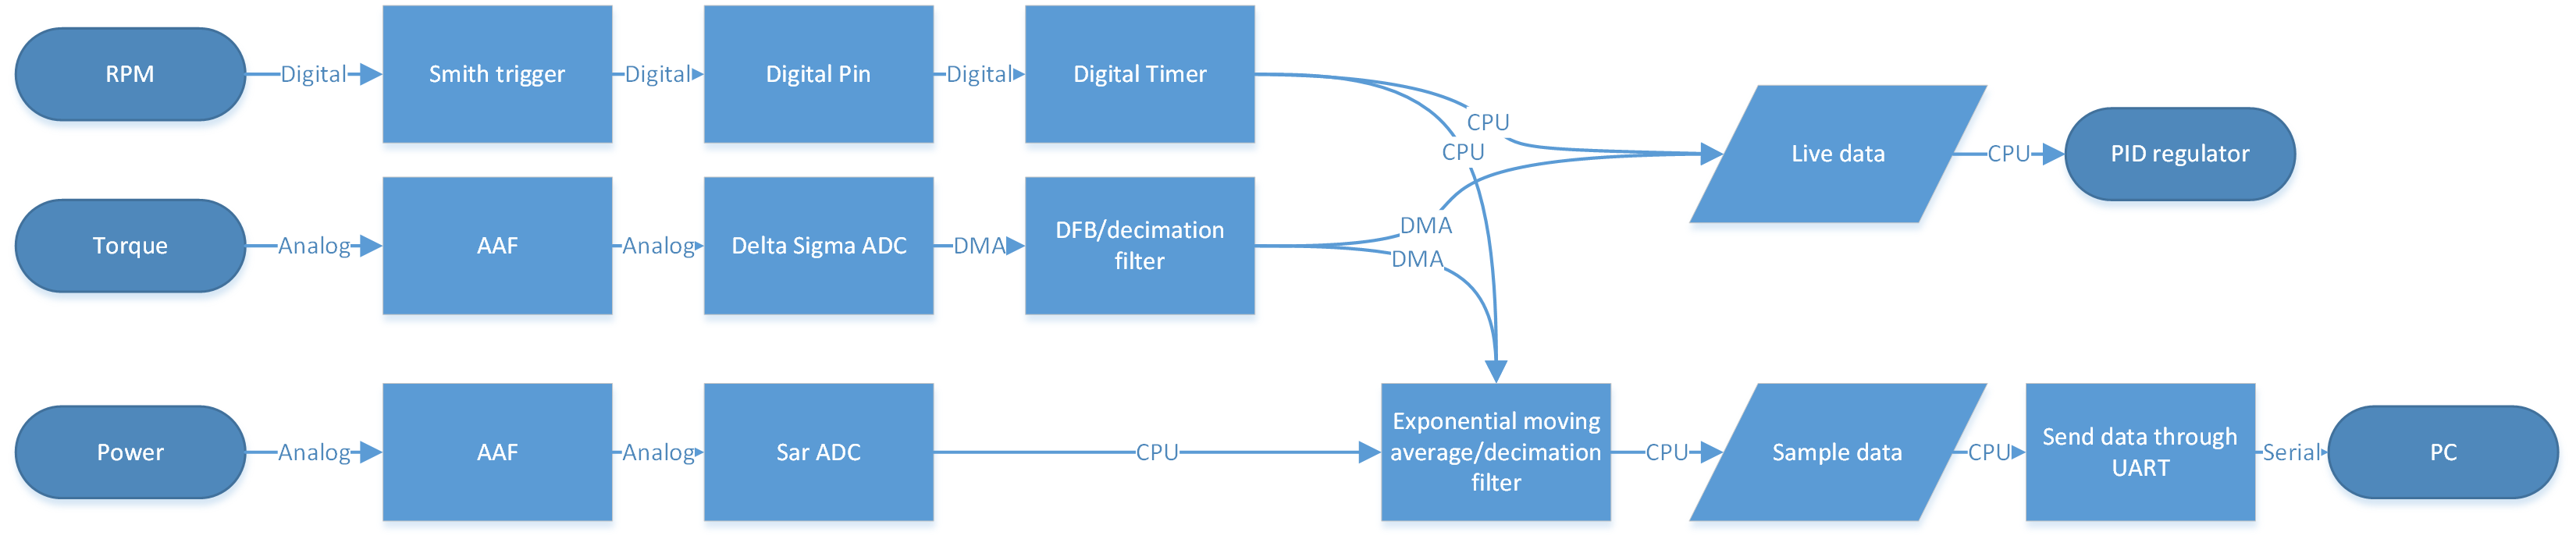
\includegraphics [width=6in]{Software/Pictures/data-flow.png}
	\caption{Rolling Road data-flow diagram.}
	\label{fig:data_flow_diagram}
\end{figure}

As seening in \ref{fig:data_flow_diagram} it can be a little hard to get a overview of the data-flow. There are sensor (four if Power count for two because it measure both voltage and current) that are our data pipes, and out there are only 2 data pipes, one that goes all the way to the main PC, this data also goes through a moving average to make a more smooth view for the user. The second output pipe has to be more fast because it is data to the PID regulator, and a too big time delay in a regulator, will make the system unstable.    

\subsubsection{Power flow}  

This flow start analog and first goes through AAF (Anti-aliasing filter) where it is converted to a digital signal with a SAR where it activates a interrupt routine where a CPU powered Exponential moving average is implemented.     

\begin{figure}[H]
	\centering
	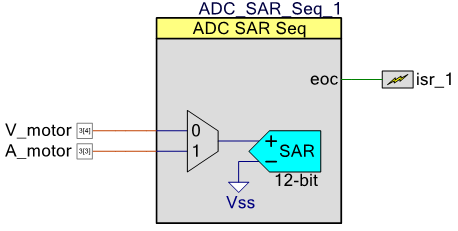
\includegraphics [width=3in]{Software/Pictures/ADC_Sar_topdesign.PNG}
	\caption{PSoC topdesign SAR ADC}
	\label{fig:ADC_SAR_topdesign}
\end{figure}

In \ref{fig:ADC_SAR_topdesign} it can see that the implementation in the top design both sample from Voltage sensor and the current sensor (Hal-sensor). 

\subsubsection{Torque flow}

This flow also starts analog and goes through a AAF but to converted the signal a Delta sigma ADC are used there the digital signal are send to DFB using DMA (Direct Memory Access). The DFB are implemented as a decimation filter to prevent aliasing then the data are moved to the PID regulator. The filter type is a 4 order IIR filter with a cut frequency at $ \SI{1}{\kilo\Hz} $. Because the PID regulator sample with a frequency of $ \SI{2}{\kilo\Hz} $.

\begin{figure}[H]
	\centering
	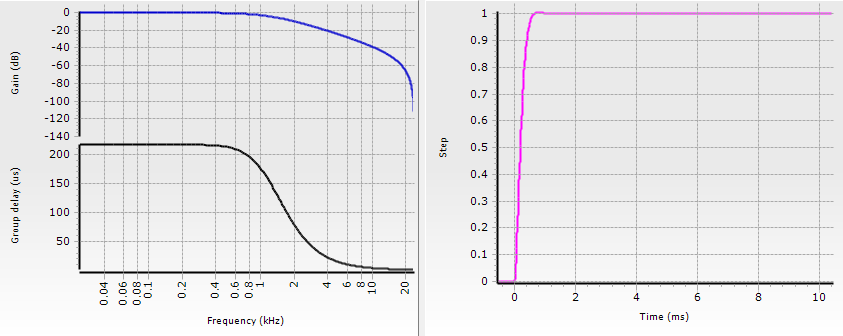
\includegraphics [width=6in]{Software/Pictures/DFB-decimation.PNG}
	\caption{DFB: decimation filter.}
	\label{fig:ADC_delsig_topdesign}
\end{figure}  

It is imported not to make too big a delay, because the data are used as a feedback to a regulator.\\
$ {(\SI{48}{\kilo\Hz})}^{-1}\times 2 + \SI{215}{\micro\s} = \SI{256.67}{\micro\s} $ \\
The delay is smaller then the regulator sampling time $ \SI{5}{m\s} $, so it should be fine, and not make the system unstable.  

\begin{figure}[H]
	\centering
	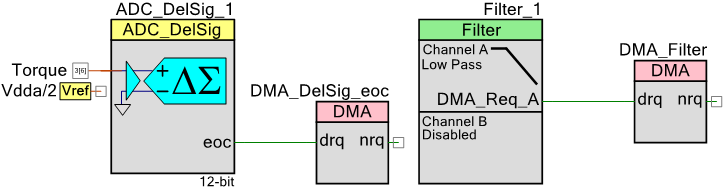
\includegraphics [width=6in]{Software/Pictures/ADC_DelSig_topdesign.png}
	\caption{PSoC topdesign of Torque sensor.}
	\label{fig:ADC_delsig_topdesign}
\end{figure}

As seen in \ref{fig:ADC_delsig_topdesign} first the torque signal is converted to a digital signal. Then it is send over to the DFB with DMA after what the signal are send to the SRAM with DMA again. 

\subsubsection{RPM flow}

This signal are a digital-signal from start to end. As a filter were are used a smith-trigger after worth it is send to a Digital timer in site of the PSoC. The digital timer use some CPU power to calculate the RPM, and save the data in the SRAM.

\begin{figure}[H]
	\centering
	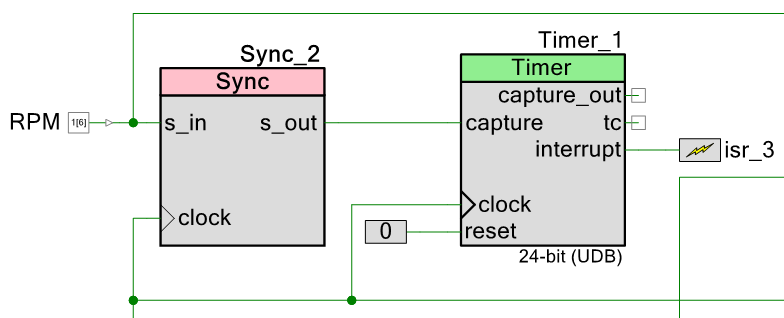
\includegraphics [width=4in]{Software/Pictures/RPM_sensor_topdesign.PNG}
	\caption{PSoC topdesign of digital timer.}
	\label{fig:digital_timer_topdesign}
\end{figure}

The timer does only measure the time between to rising edge, an from that a RPM can be measured. 

\subsubsection{output pipes}

Where are two output pipes one what are used to the PID regulator where time delay have to be as small as possible.\\
The other output are the data that are send out to the user, and here are the time delay not an imported issue because it is not used as feedback to the process. To make the data more smooth an user friendly a exponential moving average filter are implemented to there the alpha value are set to a value so it will work as a decimation filter before it are send to the PC. Because the transmission between Rolling Road and a PC are not super fast, an it also takes a lot resource to live plot the values. The reason what this process are done using CPU power, is because there are to many signals what have to been smoothen.


\lstset{language=C}
\begin{lstlisting}
CY_ISR(SAR_ADC_1)
{
	y_V_motor = (((int32)Alpha_*(int32)ADC_SAR_Seq_1_GetResult16(0))<<8) + (int32)(((int64)(256u-Alpha_)*(int64)y_V_motor)>>8) + (int32)1;
	//(8bit + 12bit + 8bit = 28bit)  +  (8bit + 28bit -8 = 28bit) ==> 28bit < 32bit ==> ok
	y_A_motor = (((int32)Alpha_*(int32)ADC_SAR_Seq_1_GetResult16(1))<<8) + (int32)(((int64)(256u-Alpha_)*(int64)y_A_motor)>>8) + (int32)1;
	//(8bit + 12bit + 8bit = 28bit) + (8bit + 28bit -8 = 28bit) ==> 28bit < 32bit ==> ok
	y_Moment = (((int32)Alpha_*(int32)Moment_temp)<<8) + (int32)(((int64)(256u-Alpha_)*(int64)y_Moment)>>8) + (int32)1;
	//(8bit + 16bit + 8bit = 32bit)  + (8bit + 32bit -8 = 32bit) ==> 32bit < 32bit ==> ok
	y_RPM = (((uint64)Alpha_*(uint64)RPM_temp)<<8) + (((uint64)(256u-Alpha_)*y_RPM)>>8) +(uint64)1;
	//(8bit + 32bit + 8bit = 48bit) + (8bit + 48bit -8 = 48bit) ==> 48bit < 64bit ==> ok
}
\end{lstlisting}

The code for exponential moving average filter, as seen are a little bit more complex then first thing, and the reason of up- and down-shifting are to make sure that no nasty rounding errors to happen. (Note: I mean nasty because it does only happen then it is some small bit values as then measure from the hal sensor beacuse it have a big range and may first work then there is more then 8 Amps.). The alpha value are made with a unsigned char there 256 is 1.\\
The alpha value should be set after have fast data are send to the PC, and should have cut frequency at the half sending frequency and how must noise there is.



